\subsection*{Problema 47}
\textbf{Enunciado:} Calcular la integral:
\begin{equation*}
\int \sqrt{4x^2 + 4x - 3} \, dx
\end{equation*}

\textbf{Solución:}
Primero, completamos el cuadrado dentro de la raíz para la expresión cuadrática.
Agrupamos los términos en $x$:
\begin{align*}
4x^2 + 4x - 3 &= 4(x^2 + x) - 3 \\
&= 4\left(x^2 + x + \dfrac{1}{4} - \dfrac{1}{4}\right) - 3 \\
&= 4\left(x + \dfrac{1}{2}\right)^2 - 1 - 3 \\
&= 4\left(x + \dfrac{1}{2}\right)^2 - 4
\end{align*}

Sustituimos esta forma en la integral original:
\begin{align*}
\int &\sqrt{4x^2 + 4x - 3} \, dx \\
&= \int \sqrt{4\left(x + \dfrac{1}{2}\right)^2 - 4} \, dx \\
&= \int 2\sqrt{\left(x + \dfrac{1}{2}\right)^2 - 1} \, dx
\end{align*}

Utilizamos la sustitución trigonométrica. 
Sea $x + \dfrac{1}{2} = \sec\theta$, de modo que 
$dx = \sec\theta \tan\theta \, d\theta$.
Además, la raíz se simplifica como:
\begin{align*}
\sqrt{\left(x + \dfrac{1}{2}\right)^2 - 1} &= \sqrt{\sec^2\theta - 1} \\
&= \tan\theta
\end{align*}

Sustituyendo en la integral:
\begin{align*}
\int &2(\tan\theta)(\sec\theta \tan\theta) \, d\theta \\
&= 2 \int \sec\theta \tan^2\theta \, d\theta \\
&= 2 \int \sec\theta (\sec^2\theta - 1) \, d\theta \\
&= 2 \int (\sec^3\theta - \sec\theta) \, d\theta
\end{align*}

Empleamos la fórmula de reducción para $\sec^3\theta$:
\begin{align*}
2 \left[ \dfrac{1}{2}\sec\theta\tan\theta + \dfrac{1}{2}\ln|\sec\theta + \tan\theta| \right. \\
\left. - \ln|\sec\theta + \tan\theta| \right] + C
\end{align*}

Simplificando los términos obtenemos:
\begin{align*}
= \sec\theta\tan\theta - \ln|\sec\theta + \tan\theta| + C
\end{align*}

Regresamos a la variable original $x$ usando $\sec\theta = x + \dfrac{1}{2}$ y $\tan\theta = \sqrt{4x^2 + 4x - 3}/2$:
\begin{align*}
&= \left(x + \dfrac{1}{2}\right)\dfrac{\sqrt{4x^2 + 4x - 3}}{2} \\
&\quad - \ln\left|x + \dfrac{1}{2} + \dfrac{\sqrt{4x^2 + 4x - 3}}{2}\right| + C
\end{align*}

\begin{figure}[H]
	\centering
	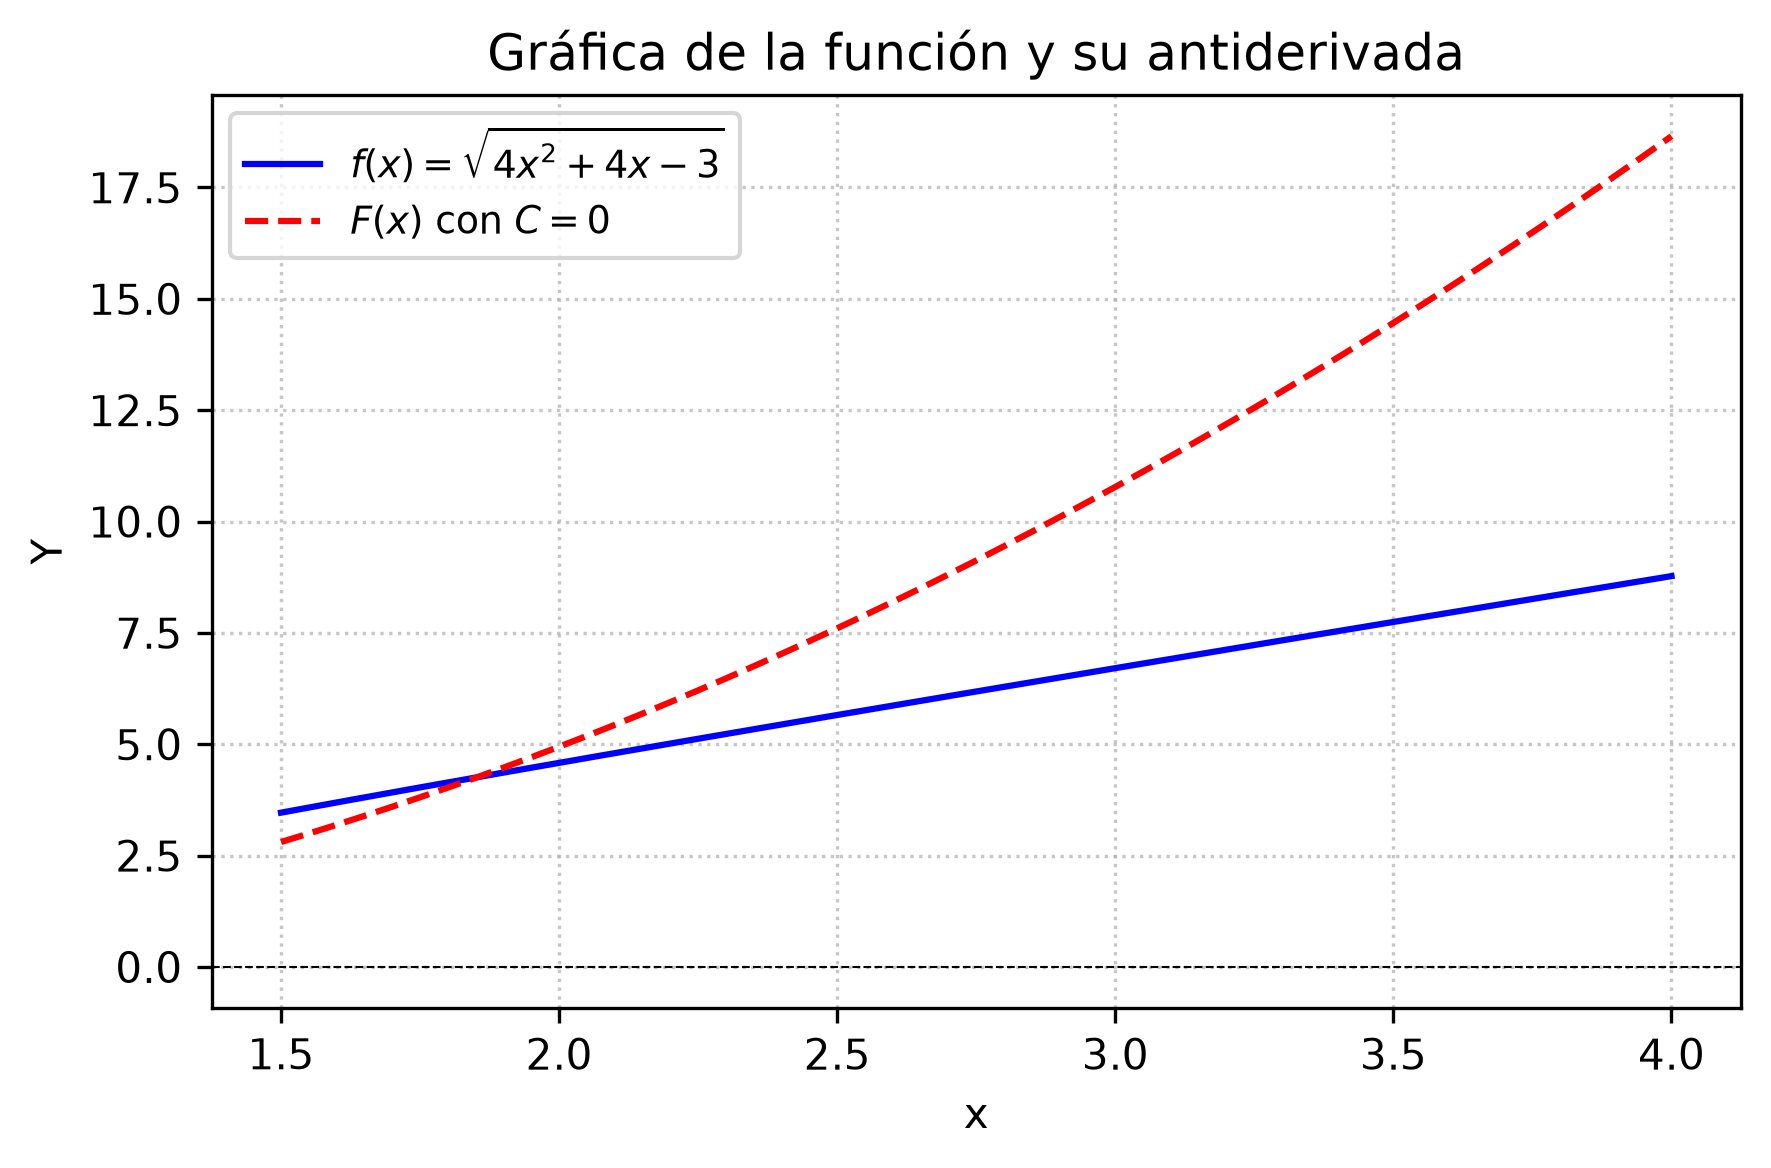
\includegraphics[width=\columnwidth]{semana_05/graficas/SEM05_P47_grafica.png}
	\caption{Representación gráfica de $f(x)$ y su antiderivada $F(x)$ evaluada para la constante de integración $C = 0$ (Problema 47).}
	\label{fig:problema47}
\end{figure}
